\section{Detailed Design and Implementation}
\label{sec:design}

\subsection{Online network-based scale plan generation}
\label{sec:design-plan}
    
\noindent
When the planner is notified to scale the parameters onto $n$ new GPUs,
it will get $s$ sources from the parameter pool, find $t$ spare GPUs as target
and generate a plan on how to send parameters from $s$ sources to 
a subset of $n$ GPUs in $t$ targets.
There are three metrics to minimize for the generation:
(1) the scale time,
(2) the plan generation time, and
(3) the interference with serving workloads.
\begin{figure}[!t]
    %    \vspace{2mm}
        \begin{minipage}{1\linewidth}
        \hspace{-1mm}
        \centering    
        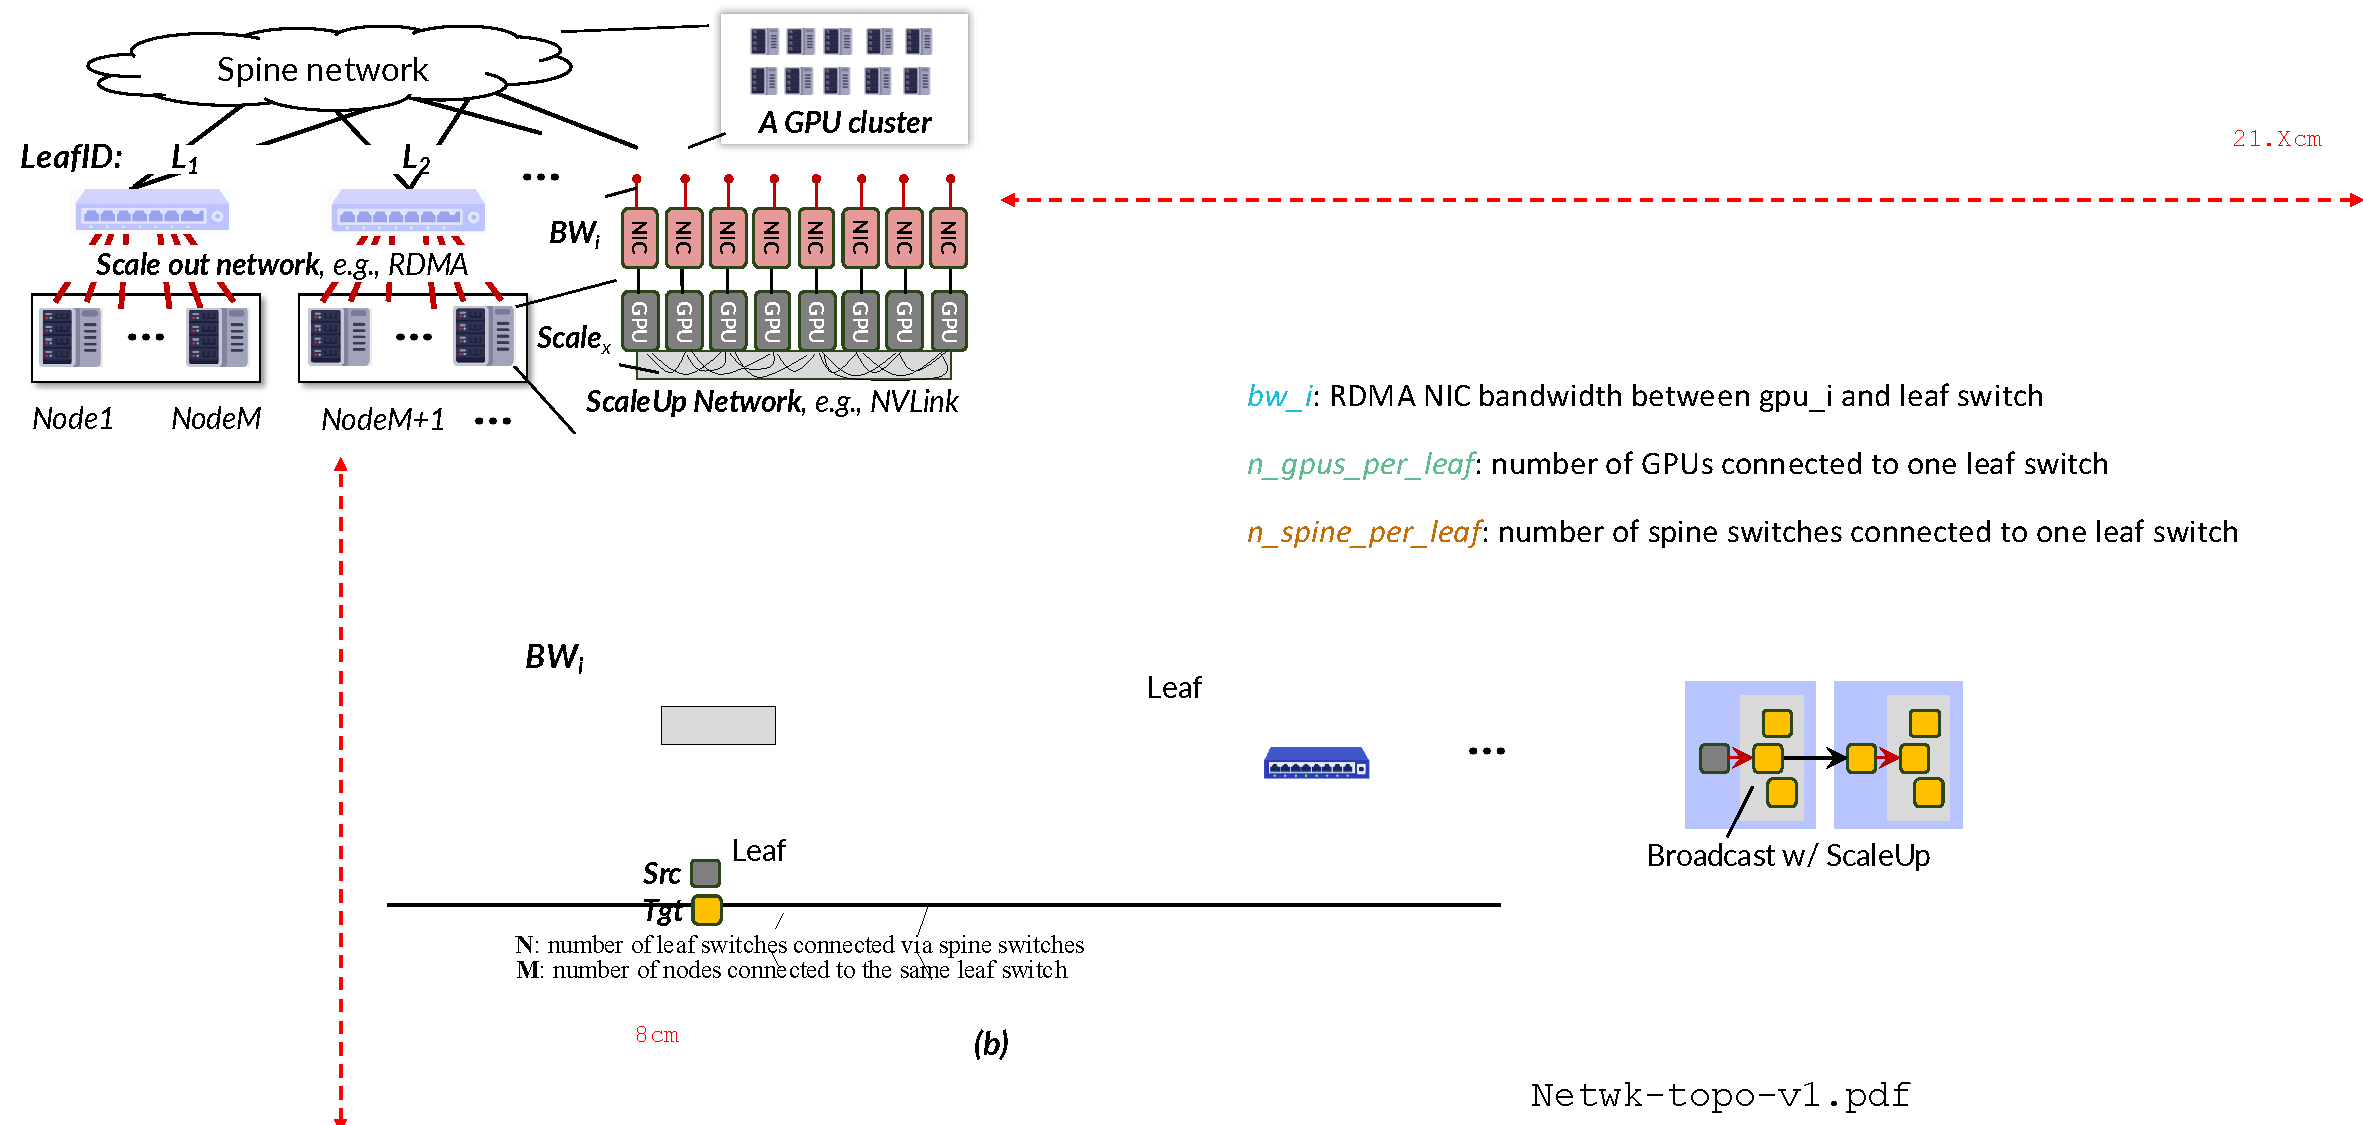
\includegraphics[width=1\textwidth, trim=0.25cm 11.45cm 23.1cm 0.25cm, clip]{figs/netwk-topo-v1.pdf} 
        \end{minipage} \\[2pt]
        \begin{minipage}{1\linewidth}
        \caption{\small{\emph{
            An illustration of how {\sys} models the network.
        }}}
        \label{fig:network-topo}
        \end{minipage} \\[-20pt]
        \end{figure} 

\stitle{Modeling the network between GPUs.\,}
Effectively generating a plan requires a model of the network between sources and targets,
which is non-trivial due to the complexity of the network topology in serving clusters.
Our model assumes a simplified scale-up and scale-out network hybrid networking,
widely adopted for GPU clusters~\cite{dellAiFabric, DBLP:conf/hoti/WangGSZH24, nvidia-compute-network}.
{\fig{fig:network-topo}} (a) illustrates the modelling. 

First, we model the GPUs connected via fast scale-up networking like NVLink
as groups of GPUs.
Such GPUs have ultra-high interconnect bandwidth (1,600-3,600\,Gbps)
so scaling within a group has negligible overhead.
On the other hand, GPUs connected via slower scale-out networking like RDMA
are more difficult to model due to a hierarchical structure.
To this end, we adopted a simple leaf-to-spine model that covers
widely deployed topologies including Clos and Rail-optimized~\cite{DBLP:conf/hoti/WangGSZH24} with different subscription ratios:
each GPU ($i$) has a $BW_i$ bandwidth connected to a leaf switch ($\text{LeafID}$),
where GPUs within the same leaf switch have a full-mesh connection,
i.e., the bandwidth between GPUs ($i$) and ($j$) is $\text{min}(\text{BW}_i, \text{BW}_j)$ with full bandwidth.
Second, leaf switches are connected to spine switches,
with inter-leaf bandwidth equal to or smaller than the intra-leaf bandwidth.
For simplicity, we don't model the spine network and rely
on upper-tier protocols like Virtual Link Trunking (VLT~\cite{DellVLTPatent2016}) and Equal-Cost Multi-Path (ECMP~\cite{RFC2992}).
to support efficient inter-leaf networking.

\iffalse
Specifically, we define the scale-up network as the high bandwidth intra-node interconnect i.e., Nvlink, 
which provides 1600/2400/3600Gbps inter-GPU connectivity for each of 8 GPUs within the scale-up network domain.
We define the scale-out fabric as the interconnect between NICs coupled with GPUs i.e., RDMA, 
which typically offers 100/200/400Gbps inter-node connectivity and enables zero-copy data exchange 
via technologies such as GPUDirect RDMA.
We assume the scale-out fabric is organized in a spine-leaf architecture, 
where only the leaf switches direct connect to NICs coupled with GPUs, 
and spine switches interconnect leaf switches (no direct leaf-to-leaf connection).
This modeling supports different and scalable network topologies with various subscription ratios, 
e.g., the leaf switch can be a ToR switch connecting 32 GPUs, 
or a set of rails connecting 256 GPUs. 
Finally, we assume the spine layer switches employ Virtual Link Trunking (VLT) and Equal-Cost Multi-Path (ECMP) 
protocols for efficient inter-leaf switching and routing, and thus the leaf-to-leaf aggregated bandwidth is no less than 
the aggregated bandwidth between a leaf switch and a single node.
\fi

\begin{figure}[!t]
    %    \vspace{2mm}
        \begin{minipage}{1\linewidth}
        \hspace{-1mm}
        \centering    
        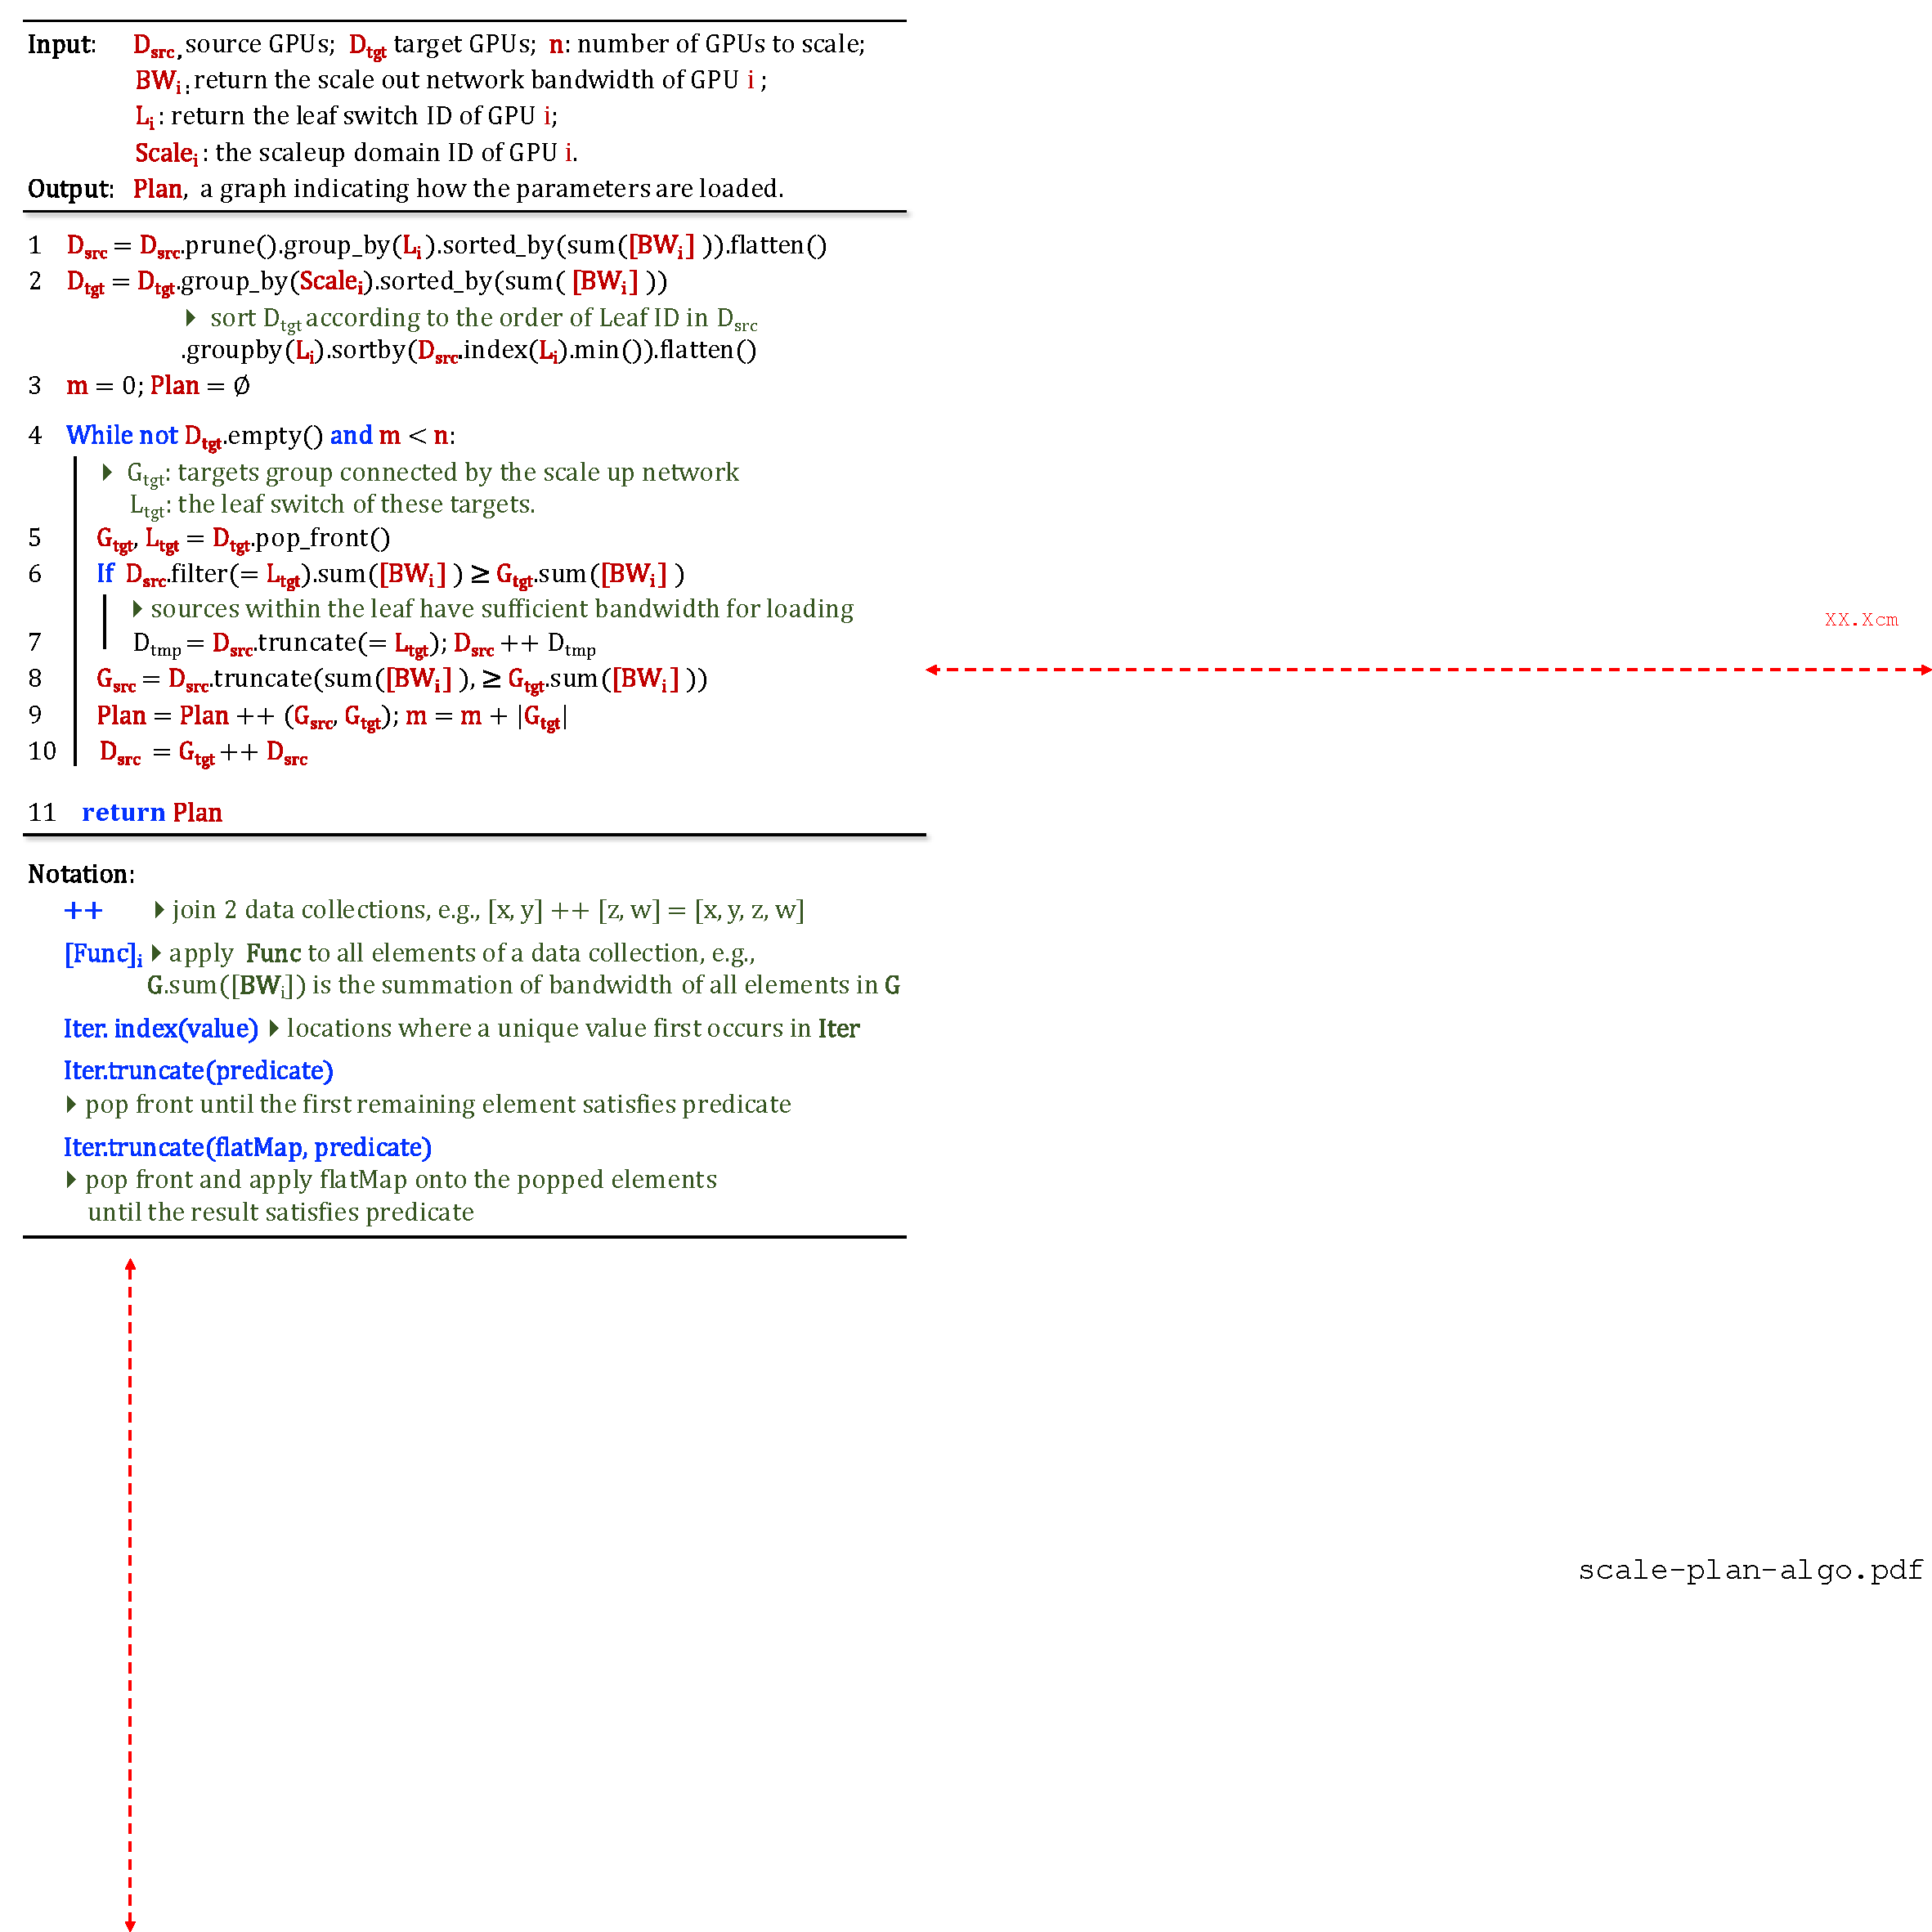
\includegraphics[width=1\textwidth, trim=0.25cm 14cm 21cm 0.25cm, clip]{figs/scale-plan-algo.pdf} \\[1pt]
        \end{minipage} \\[3pt]
        \begin{minipage}{1\linewidth}
        \caption{\small{\textit{
            The pseudocode of the plan generation algorithm.
        }}}
        \label{alg:alg-plan}
        \end{minipage} \\[-15pt]
        \end{figure}         

\stitle{Multicast-chain-based greedily plan generation. \,}
To quickly generate the plan online, we use a three-step greedy algorithm
as shown in Algorithm~\ref{alg:alg-plan}.
First, we prune the sources to avoid any interference with serving workloads (Line 1).
Second, we group targets connected with scale-up networking like NVLink as
a group (Line 2) such that we can leverage the NVLink broadcast
to efficiently realize parallel sharded parameter transfer,
see {\fig{fig:parallel-shards}} and described below.
Finally, we form multiple serial broadcast chains (Line 3--10) 
to generate the plan.

\iffalse
First, we group all targets connected via NVLink 
into a group (Line 1). The parameters will only load to one instance in the group,
while others receive the parameter through NVLink broadcast. 
This reduces complexity without sacrificing speed,
because the NVLink broadcast time can be overlapped with RDMA transfer.
For example, for a Llama2-7B model, 
%its average TTFT and TBT are \TODO{xx} and \TODO{yy} on \TODO{xx} workloads,
%so a scale speed of \TODO{xx} is sufficient to meet the SLO requirements (see \textsection{\ref{sec:bg-motiv}}).
%Broadcasting with NVLink only takes \TODO{xx}, which clearly satisfies our requirement.
Transferring it with 200\,Gbps RDMA would take 650ms, 
while broadcasting it with NVLink only takes 105ms in practice. 
\DY{ADD ptr to parallel sharded parameter transfer}
We have also developed an optimization to parallelly transfer parameters to 
multiple instances within the same group in a sharded way, 
which is discussed in ~\ref{sec:design-shard}

While NVLink can dramatically improve multicast speed, 
it is not always applicable because: 
(1) GPUs with NVLink are typically used to form a single instance for large models
(e.g., Llama2-70B, Qwen-72B) and 
(2) clusters may lack NVLink (see {\fig{fig:gputopo}} (b)).

Second, to avoid network interference, 
we remove links between sources and targets that could cause bandwidth contention, 
guided by the serving workloads (Line 2). 
For example, in PD  disaggregation, 
only the prefill instance will send data to the decode instance. 
Since these flows are static throughout the inference, we can systematically
prune them before generating the plan. 
Our prune is based on whether a source has outcast link:
e.g., if $s_i$ also sends outcast network, 
we will delete $s$ from the sources.
\fi
 
        
\begin{figure}[!t]
    %    \vspace{2mm}
        \begin{minipage}{1\linewidth}
        \hspace{-1mm}
        \centering    
        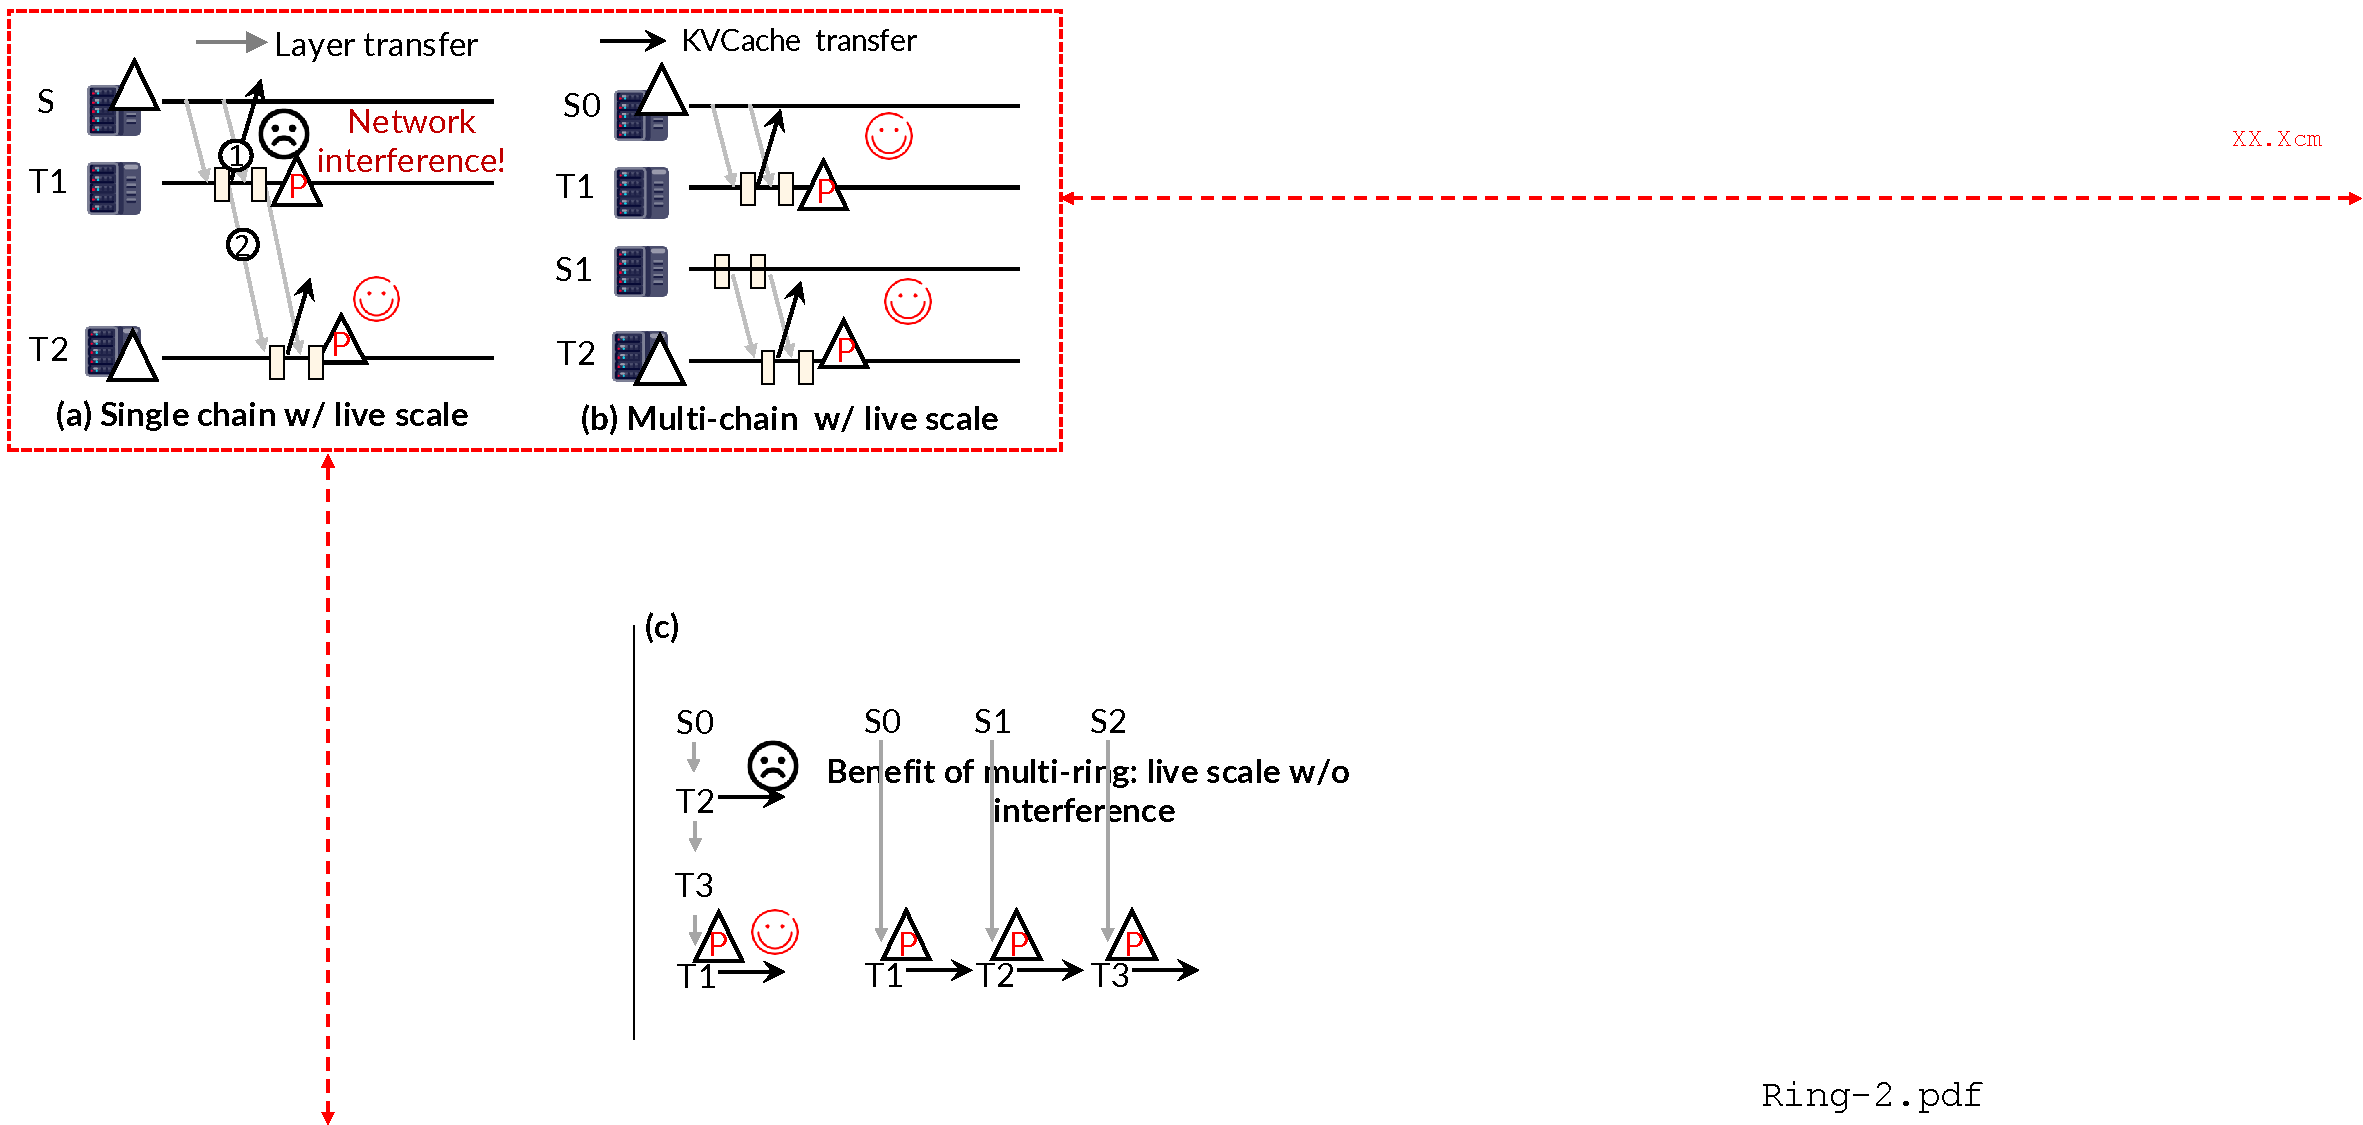
\includegraphics[width=1\textwidth, trim=0.25cm 11.6cm 23cm 0.25cm, clip]{figs/ring-2.pdf} \\[1pt]
        \end{minipage} \\[4pt]
        \begin{minipage}{1\linewidth}
        \caption{\small{\emph{
            An illustration of why multiple chains are better especially 
            under live scaling.
        }}}
        \label{fig:ring-2}
        \end{minipage} \\[-15pt]
        \end{figure}          

\begin{figure}[!t]
    %    \vspace{2mm}
        \begin{minipage}{1\linewidth}
        \hspace{-1mm}
        \centering    
        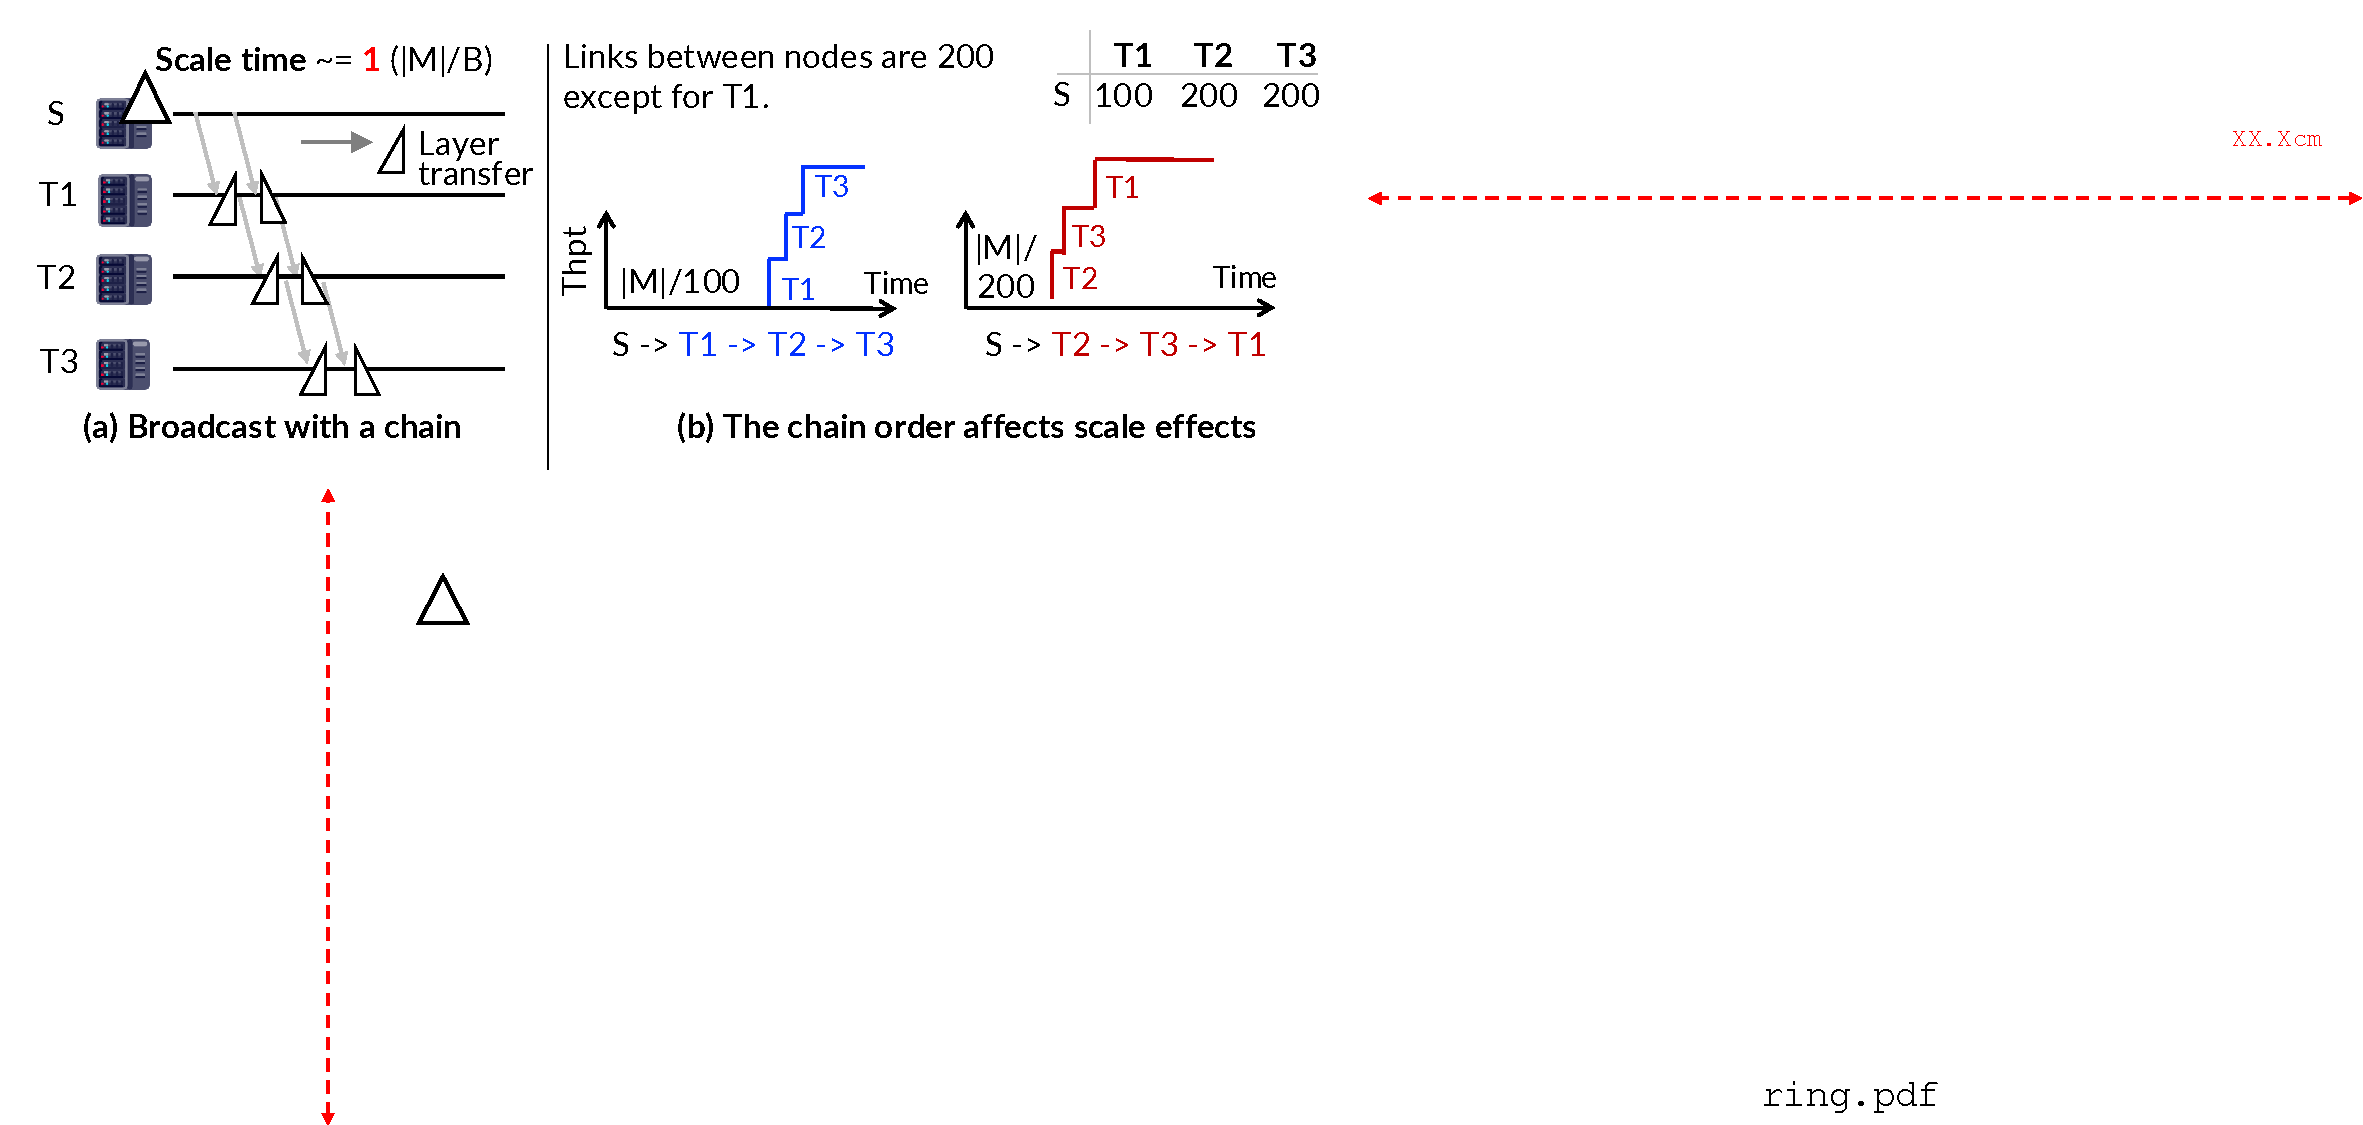
\includegraphics[width=1\textwidth, trim=0.25cm 11.6cm 17.5cm 0.25cm, clip]{figs/ring.pdf} 
        \end{minipage} \\[7pt]
        \begin{minipage}{1\linewidth}
        \caption{\small{\emph{
            An illustration of 
            (a) why chain is friendly to broadcast with huge bandwidth requirement and
            (b) why we chooses a specific chain order. 
            $|M|$ is the model size and $B$ is the slowest network bandwidth between 
            nodes in a chain.
        }}}
        \label{fig:ring}
        \end{minipage} \\[-10pt]
        \end{figure} 

Specifically, a serial broadcast chain is formed by a set of source and target nodes,
i.e., $S \rightarrow T_1 \rightarrow T_2 \rightarrow ... \rightarrow T_n$.       
Note that a node in a chain may have multiple GPUs. 
Such a chain has a nice property that it is optimal in bandwidth-intensive transfer like 
model scaling, because the overall transmission time is irrespective of the instances scaled with such a chain.
As shown in {\fig{fig:ring}} (a), 
when T1 receives the first layer,
T1 immediately forwards it to T2.
Meanwhile, $S$ will continue to send the second layer to T1,
so the time of sending the first and second layer is overlapped.


While a serial chain is sufficient for efficient parameter broadcasting for nodes that are connected
with the same bandwidth links,
multiple chains are necessary in a leaf-spine network where inter-leaf bandwidth may vary
and in our live scale setup.
This is
because (1) multi-chain avoids relatively slow inter-leaf communications if each leaf switch
has sources and targets (Line 6--7),
and (2) it enables more interference-free live scaling especially in PD disaggregation setting.
{\fig{fig:ring-2}} illustrates the latter:
suppose we want to scale up two prefill instances in a live manner,
the KVCache will be transferred to the decode instances once prefill is done.
With a single chain, only $T2$ can join the live scale without network interference,
because at $T1$, the KVCache transfer (\ding{192}) interferes with the
parameter forward traffic (\ding{193}).
With two chains backed by two parameter sources (b), both $T1$ and $T2$
can live scale without interference.

Note that the order of nodes in the chain is important:
we chose a decreasing order with respect to the aggregated link speed between nodes (Line 2, 5).
This is because 
sending to nodes with higher bandwidth achieves a faster increase in the serving throughput. 
As shown in {\fig{fig:ring}} (b): 
suppose the source ($S$) sends parameters to $T2$ twice as fast as $T1$.
A chain order of $S \rightarrow T2 \rightarrow T1$ is better than $S \rightarrow T1 \rightarrow T2$
because the downtime of $T2$ is only half.
Note that the source can be a group of GPUs because GPUs typically have dedicated network cards
in our setup.

\iffalse
Another benefit of decreasing aggregated bandwidth order is that the aggregated source bandwidth 
remains higher in our plan (Line 8, 10). In the aforementioned example, after the first hop 
$S \rightarrow T2 \rightarrow T1$ will have higher source bandwidth since $T2$ has higher bandwidth than $T1$.
\fi
\iffalse
Multi-chain design can also reduce the upstream network traffics between leaf switches 
within the spine tier according to our network modeling.
We keep chians spanning within the same leaf switch as much as possible  
\DY{mistack: for all pairs of leaf switches, the chain does not across leaves at most once.}
by giving priority to select sources within the same leaf as target (Line 6-7). 
If there is no eligible sources, the scaling plan will add a leaf-to-leaf traffic 
but span sources within target leaf switch (Line 10). 
Since we select targets in a bandwidth decreasing order (Line 2, 5), the successive targets within the same leaf 
can leverage this newly spanned source.
\fi

\begin{figure}[!t]
    %    \vspace{2mm}
        \begin{minipage}{1\linewidth}
        \hspace{-1mm}
        \centering    
        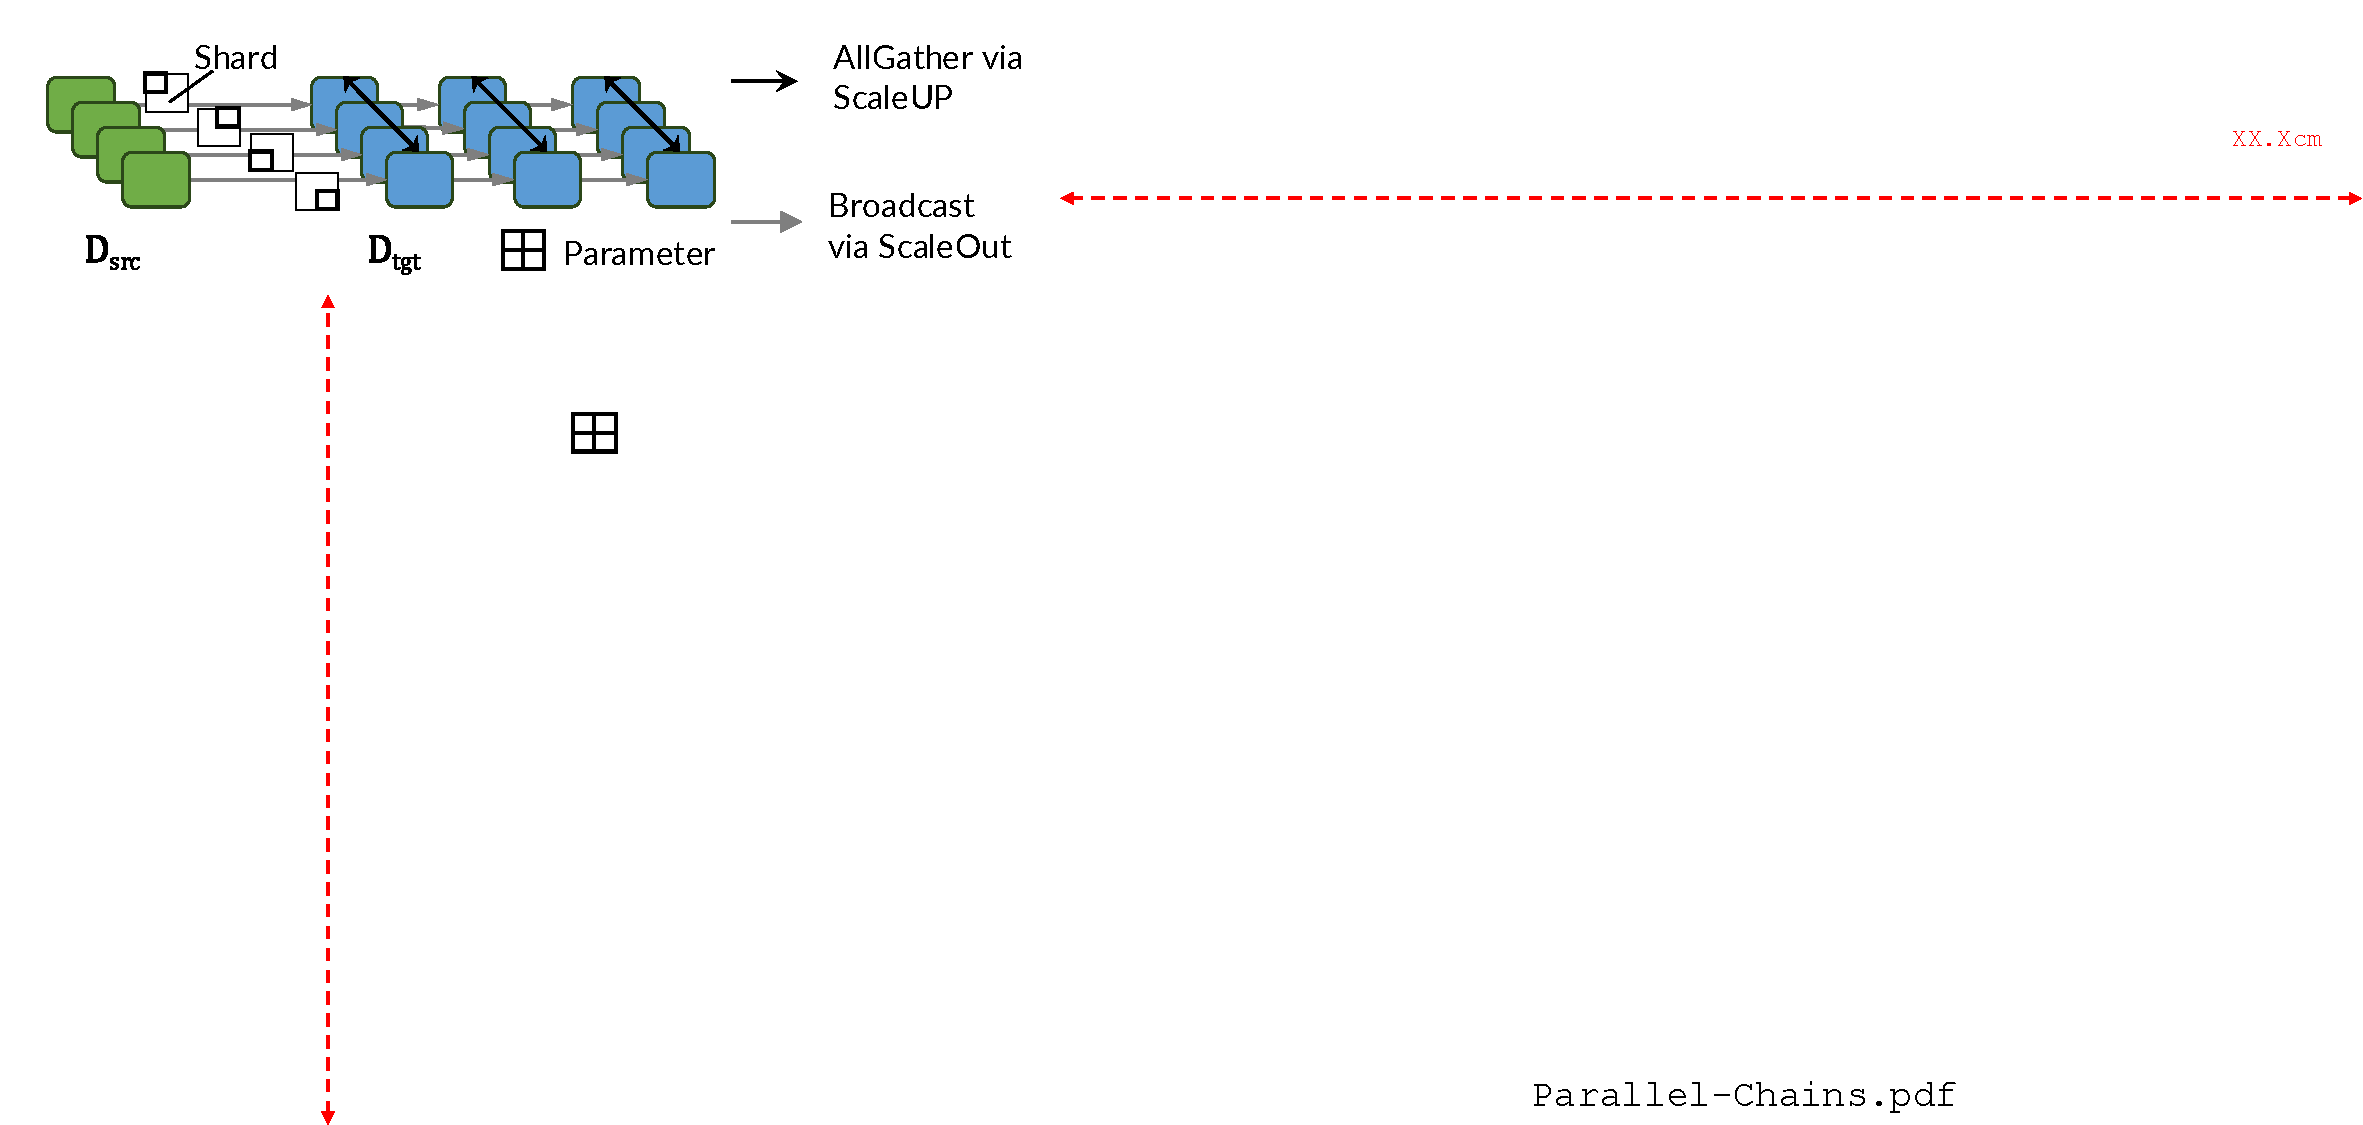
\includegraphics[width=1\textwidth, trim=0.25cm 14.2cm 22.5cm 0.25cm, clip]{figs/parallel-shards.pdf} \\[1pt]
        \end{minipage} \\[4pt]
        \begin{minipage}{1\linewidth}
        \caption{\small{\emph{
            An illustration shareded parameter transfer with scale up network. 
        }}}
        \label{fig:parallel-shards}
        \end{minipage} \\[-15pt]
        \end{figure}       

\stitle{Optimization: parallel sharded parameter transfer from multiple sources. \,}
\label{sec:design-shard}
For a broadcast chain where the source and target contain GPUs with duplicated parameters,
we further leverage the scale-up network to parallelize a transfer link.
{\fig{fig:parallel-shards}} shows a concrete example.
Suppose the source and target nodes have four GPUs each.
For such a transfer, each source GPU only needs to forward 1/4 of the sharded parameters to each target GPU,
where the target GPUs can use NVLink-based AllGather to get the full parameters.
This reduces the scaling time to 1/4 as the NVLink AllGather time is negligible.


\subsection{Efficient live autoscaling with ZigZag scheduling}
\label{sec:design-pp}

\nospacestitle{Selecting instances for live scaling. \,}
After getting the chains from Algorithm~\ref{alg:alg-plan},
we select instances to participate in live autoscaling
based on the following criteria:
(1) the necessity of live autoscaling,
i.e., when a stop-the-world scaling will cause SLO violation and
(2) the presence of overloaded instance that can cooperate.
Both are readily available:
(1) we can profile the relationship between load speed and SLO violation
 in {\fig{fig:motiv-scale-speed}} for the judgement and
(2) autoscaling is typically triggered when the system is overloaded.
Thus, for each overloaded instance, we
will identify an instance in the chain that satisfies (1),
typically the tail instances in the chains as it has the slowest link.

\stitle{Live autoscale protocol with paired instances. \,}
Suppose we have selected a new instance (inst.1) to offload computations 
from an overloaded instance (inst.0). 
To begin live autoscaling, 
we use a three-step transition protocol:
(1) Once inst.1 starts loading parameters, 
we redirect all queued and new requests from inst.0 to it for execution. 
The redirection time is negligible because the request payloads are much smaller than the model. 
(2) After the first layer is loaded on inst.1, 
it begins executing the first layer of all requests. 
Note that during the loading of the first layer, 
inst.0 remains active by processing its pending requests. 
Finally, when the model has completed loading on inst.1 (3), 
requests will be re-distributed evenly between 
both instances.

\begin{figure}[!t]
    %    \vspace{2mm}
        \begin{minipage}{1\linewidth}
        \hspace{-1mm}
        \centering    
        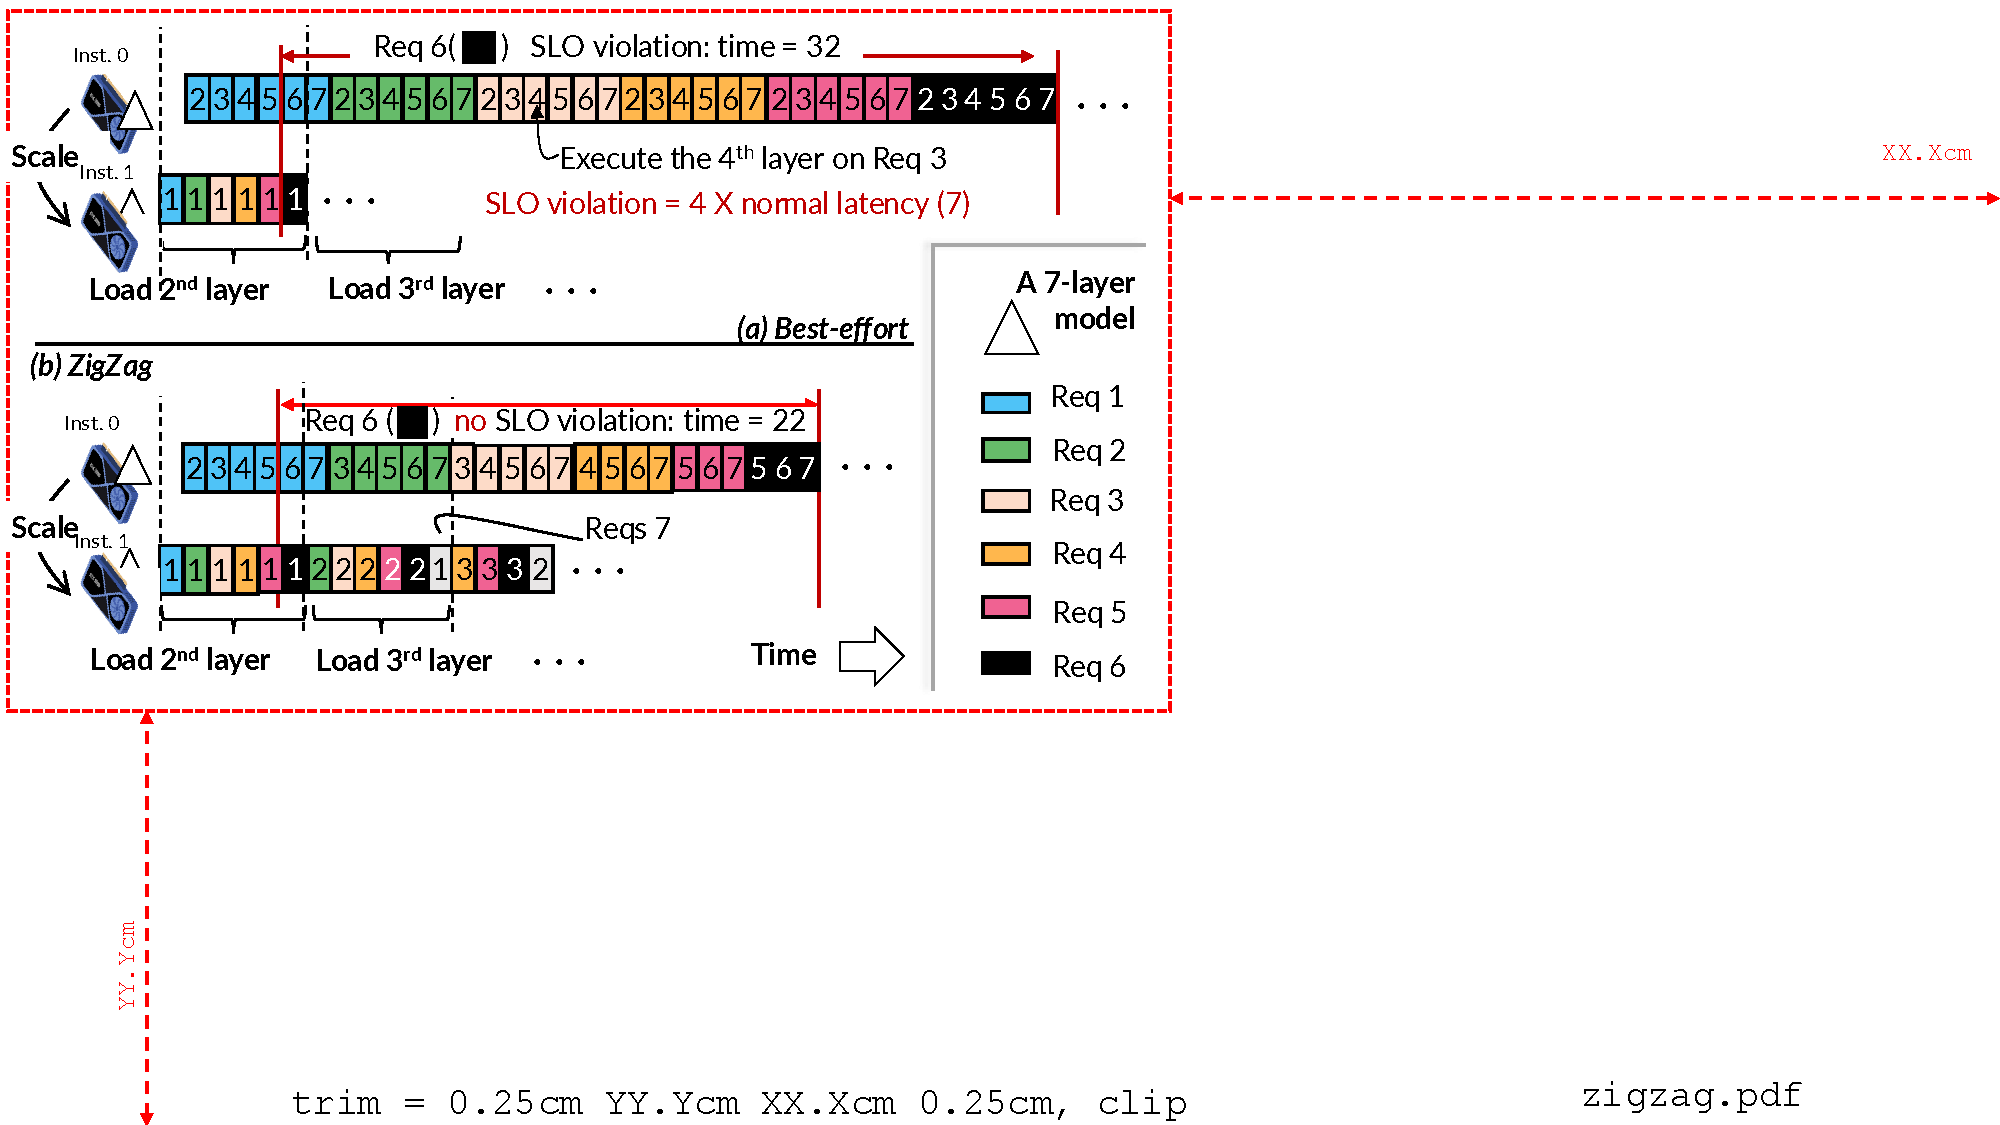
\includegraphics[width=1\textwidth, trim=0.25cm 7.1cm 14.2cm 0.25cm, clip]{figs/zigzag.pdf} \\[1pt]
        \end{minipage} \\[3pt]
        \begin{minipage}{1\linewidth}
        \caption{\small{\textit{
    An illustration of the necessity of ZigZag scheduling.
    Note that the execution starts when the first layer has been loaded to instance 1 (inst.1).
    Our example assumes the time of loading a layer can perform 6-layer computations.
        }}}
        \label{fig:zigzag}
        \end{minipage} \\[-15pt]
        \end{figure} 

\stitle{The scheduling problem. \,}
A key issue to address in the above (3) is 
how to best utilize inst.1 to maximize the goodput during live autoscaling. 
Specifically, we should decide a pipeline configuration for each request batch,
i.e., how many layers to execute on inst.1 and inst.0, respectively.
\iffalse
An alternative solution---waiting until half of the layers 
are loaded on GPU1 before starting execution---is also suboptimal, 
as it wastes half of the model load time.
\fi
One naive policy is best-effort:
for each batch, we execute as many layers as possible on inst.1 (not exceeding half)
and execute the rest on inst.0.
While it adapts configurations with model loading,
we found it is suboptimal because
inst.1 has limited serving capacity during initial loading,
so most requests are still queued at inst.0, causing SLO violations.
{\fig{fig:zigzag}} (a) shows a concrete example
of a 7-layer model executed with the best-effort scheduling.
The load time of one layer can do 6-layer computations,
a common setup (e.g., Llama2-7B model with a moderate batch size of 2000 prefill tokens under 200\,Gbps RDMA network).
Thus,
before the second layer has been loaded to inst.1,
the current request batches (req 1--6) can only use a $(1,6)$ pipeline configuration.
However, request 6 will suffer from SLO violation
due to waiting for requests 1--5 to be completed on inst.0,
as their execution time has reduced a little due to the imbalanced loads.
%The reason is that requests 1--5 has insufficient reduced execution time 
%due to an unbalanced pipeline configuration.

\stitle{The ZigZag scheduling. \,}        
To address this issue, our observation is that
by delaying request scheduling on inst.0,
inst.1 will have more layers coming,
opening opportunities to balance the workload between instances.
{\fig{fig:zigzag}} (b) shows this:
After requests 2--5 have been executed on inst.1,
we delay their execution on inst.0 and wait for the second layer to come.
This allows us to adopt a more aggressive pipeline configuration $(2,5)$ for them.
Note that the delay won't waste GPU because we can schedule pending requests (e.g., 6).
After the second layer has been loaded,
inst.1 can come back (thus, in a ZigZag way) to execute the second layer of requests 2--5.
Thus, the second layer execution of requests 3--6
is overlapped with the execution of layers 3--6 for request 2.
Thanks to this overlap, the overall inference time of request 7
decreases from 32 to 22, now within the SLO.

The above ZigZag scheduling can be formulated as follows.
Assuming a first-come-first-serve (FCFS) scheduling policy,
the de facto for serving~\cite{vllm,DBLP:journals/corr/abs-2404-09526,DBLP:conf/osdi/YuJKKC22}.
For ease of presentation,
we first assume non-LLM and then extend to LLM in \textsection{\ref{sec:design-llm}}.
The scheduling has two parts:

\emph{\uline{(1) Pipeline configuration. }}
Given $N$ request batches with equal execution time,
we first determine the pipeline configuration ($\text{T}_i, \text{S}_i$) for them,
where $\text{T}_i$ and $\text{S}_i$ are the number of layers
to be executed on the target and source GPU for request $i$,
respectively.
The goal is to minimize the average latency,
which can be formulated with the following Integer Linear Program (ILP): \\[-5pt]
\[
 \text{Latency}_\text{avg} = (\sum_{req=1}^{N} \sum_{i=1}^{req} \text{S}_{i}) / N
\] \\[-3pt]
\noindent
To see why such a formula holds, consider the example in {\fig{fig:zigzag}} (b).
Each request's latency is the time the source instance finishes its part of the computation,
which includes its own execution time and the sum of its previous requests' time (queueing time).
We only need to consider previous requests because they are executed in a FIFO order.
In our example, request 3's latency is 17 (12 for requests 1 and 2's execution and
5 for its own).
For non-LLM, the execution time of each layer is the same if the batch size is the same.
Note that we omit the activation transfer latency since it is negligible.

The problem has the following constraints: 
\begin{mini}
    {}{\text{Latency}_\text{avg}}{}{} \\[-20pt]
    \addConstraint{\text{S}_{i} +  \text{T}_{i} = L, \quad \forall i \quad \text{Pipeline limit \bf{(C1)}}}{}  \vspace{-10pt}
    \addConstraint{\sum_{j=1}^{i} \text{T}_j  \le \sum_{j=1}^{i-1} \text{S}_j,\forall i > 1 \quad \text{Pipeline dependency \bf{(C2)}}}{} \vspace{-10pt}
    \addConstraint{\text{Time}_{l} \ast \text{T}_i \leq \sum_{j=1}^{i-1} \text{T}_j + (N-i+1) \times (\text{T}_i - 1)} \vspace{-15pt}
    \addConstraint{\forall i > 1 \quad \text{Load limit \bfseries (C3)}}{}
    \label{eq:pp-config}
  \end{mini}
\noindent
\textbf{C1} ensures that the pipeline should be fully executed. 
\textbf{C2} states pipeline dependency: 
when the source instance executes request $i$'s $S_i$ layers, 
the target instance must finish the execution of $T_i$. 
The start execution time of request $i$ on the source is 
$\sum_{j}^{i-1} \text{S}_j$.
The finish time of $i$ on the target instance is $\sum_{j}^{i-1} \text{T}_j + \text{T}_i$,
which simplifies to $\sum_{j}^{i} \text{T}_j$. 
Finally, \textbf{C3} ensures that once the target instance request's $i$'s $T_i$ layers, 
all these layers must be loaded, where $\text{Time}_l$ is 
the time to load one layer normalized to the execution time of one layer in pipeline. 
%The term $\sum_{j=0}^{i-1} \text{T}_j$ indicates the load time can be 
The term $(N-i+1) \times (\text{T}_i - 1)$ indicates that the load time can be 
overlapped with executing of the succeeding requests of $i$. 
%the execution time of preceding requests, 
%while $(N-i+1) \times (\text{T}_i - 1)$ states the max allowed execution time of succeeding 
%requests without violating the FCFS requirement. 

While solving this ILP is NP-hard, it remains manageable (less than 40\,ms to solve for Llama3-8B)
because models typically have only a few dozen layers. 
Additionally, we only need to configure the pipeline for the batches of requests 
executed during parameter loading, which is a dozen of so in practice.
Nevertheless, 
to further eliminate the solving time for models with more layers (e.g., 80 layers for Qwen-72B),
we also derived an ILP-free method that we described below. 

\begin{figure}[!t]
    %    \vspace{2mm}
        \begin{minipage}{1\linewidth}
        \hspace{-1mm}
        \centering    
        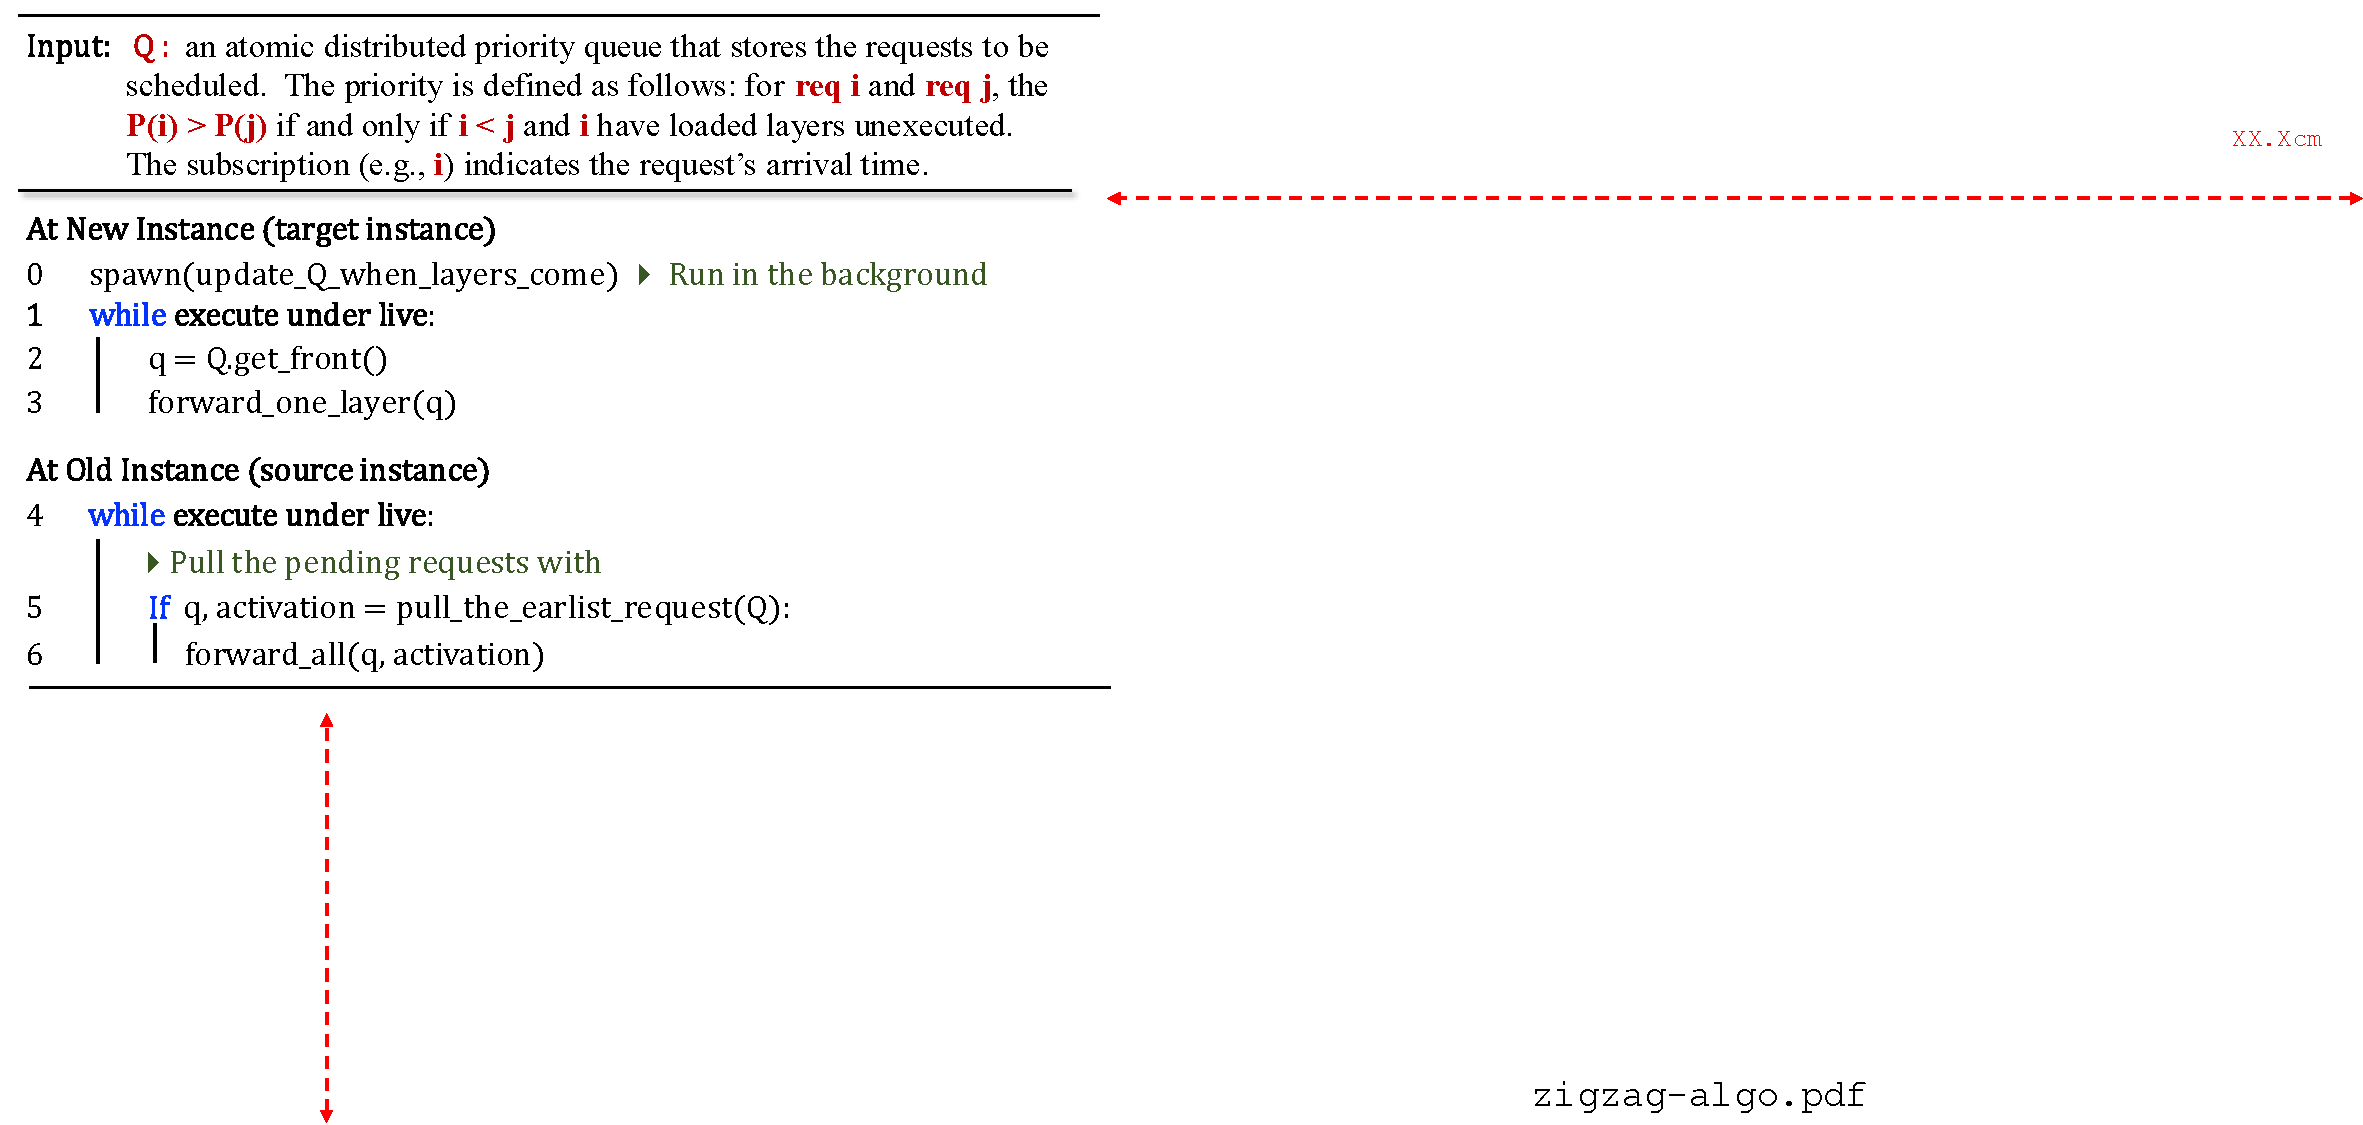
\includegraphics[width=1\textwidth, trim=0.25cm 6.99cm 21.3cm 0.25cm, clip]{figs/zigzag-algo.pdf} \\[1pt]
        \end{minipage} \\[3pt]
        \begin{minipage}{1\linewidth}
        \caption{\small{\textit{
            The pseudocode of the ILP-free ZigZag scheduling.            
        }}}
        \label{fig:zigzag-algo}
        \end{minipage} \\[-15pt]
        \end{figure} 

%\vspace{0.5ex}
\emph{\uline{(2) Scheduling requests in an ILP-free ZigZag way. }}
Specifically, we found that by delaying sending the requests on the
source instance
and letting the target instance execute the requests once it is free,
we can achieve ZigZag scheduling without solving the ILP.
{\fig{fig:zigzag-algo}} shows the pseudocode of how we schedule the requests on both instances.
The new instance maintains a priority queue (that can be pulled by the source instance via RPC)
for all requests,
where the priority is defined by (1) the FCFS order and
(2) requests with next-to-execute layer loaded coming first.
Once the new instance has executed one layer (Line 3),
we keep the executed request in the queue so it can be scheduled back once
more layers are loaded.
The requests are scheduled on the source instance only if
it is not overloaded, i.e., has no pending requests (Line 5).
Thus, if the source instance is busy,
the request will still be executed on the target instance.

\iffalse
Based on the pipeline configuration, 
the scheduler on the new instance rehearses request execution. 
To achieve FIFO, we use a priority queue for all requests. 
A problem is that when executing a specific request, the new instance may lack its required layers. 
These requests are moved to a pending queue. 
For timely rescheduling these requests, 
we implement a preemption mechanism: 
whenever a new layer loads, 
we scan the pending queue and execute all requests that require that layer. 
\fi


\subsection{Global parameter pool and scaling policy}
\label{sec:design-others}

\nospacestitle{Global parameter pool and local memory cache. }
Our global parameter pool tracks the locations of the model parameters across deployed GPUs and host CPUs
with local memory cache.
To ensure at least one copy of the model parameters is available in the
memory of GPU or host at the cluster scale,
during system initialization,
we distribute one copy of the model's parameters evenly
to the CPU hosts and track their locations at a centralized manager.
When a model is deployed to or reclaimed from a GPU,
we further update the locations in the manager,
and reclaim/reload cached copies on the host cache.

\iffalse
The parameters at the local cache of the hosts 
will be stationary except under failures (described below).
Since we only cache one copy, 
we don't need an eviction policy~\cite{DBLP:conf/usenix/Romero0YK21,DBLP:journals/corr/abs-2401-14351},
because memory from all the hosts (1.5\,TB each) is sufficient to store all the models.
Note that when a model is deployed on an instance's GPU(s), we can 
even drop its cached copy at the host. 
In this paper, we focus on the autoscaling mechanism, 
so we use a simple distribution policy that ensures exactly one copy exist 
for each model across the machines managed. 
While replicating the parameters enable more live autoscaling opportunities (e.g., see {\fig{fig:ring-2}}),
it comes at the cost of extra memory usage, and we leave it as future work.
\fi

\stitle{Scaling policy. \,}
Our paper focuses on the autoscaling mechanism,
which is orthogonal to the autoscaling policies,
including
collecting workload metrics with workload monitoring
and determining how many new instances to scale based on these metrics.
Our current implementation follows prior works~\cite{DBLP:conf/osdi/SunHZXZL024,K8S-HPA}
that first records the serving loads with tokens per second and KVCache usage globally.

For scaling up,
when the average monitored load surpasses a pre-defined upper bound,
we allocate sufficient instances to meet that demand.
The upper bound can be derived by profiling the average serving load per-instance offline.
We leave a more detailed explanation in another paper. 
For scaling down,
we follow previous works'\cite{DBLP:conf/usenix/Romero0YK21,DBLP:journals/corr/abs-2401-14351}
timeout-based policy:
when the average monitored load falls below a lower bound in a time window,
we shut down some instances and revoke all GPUs assigned to them.
Given {\sys}'s rapid autoscaling capabilities,
we adopt an extremely short sub-second level timeout.

\subsection{Specializations and optimizations for LLM}
\label{sec:design-llm}

\noindent
While most techniques described above work for all models following a
layer-by-layer architecture,
the unique characteristics of LLMs especially for LLMs served with PD disaggregation
require several specializations and optimizations.

\stitle{Retrofitted live pipeline scheduling formulation. \,}
Our formulas and constraints described in \textsection{\ref{sec:design-pp}} cannot be directly applied
to LLMs
because the prefill and decode time of a layer is approximately
linear to the total batched token size~\cite{DBLP:conf/isca/PatelCZSGMB24,DBLP:journals/corr/abs-2404-09526}.
For prefill-only live scheduling, e.g., autoscaling a prefill instance in PD disaggregation,
we fix the formulation by adding
a regulation parameter for each request batch by profiling its execution time with the counts,
similar to a priori work~\cite{DBLP:journals/corr/abs-2404-09526}.
A more tricky case involves handling decoding,
e.g., when scaling instances that combine prefill and decode,
or scaling a decode instance in PD disaggregation.
The complexity arises because decode batch size changes dynamically
due to its auto-regressive nature.
Fortunately, our ILP-free scheduling method can also work for decoding.

\stitle{Supporting PD colocation. \,}
We seamlessly support PD colocation since a PD-colocated instance 
is a normal model instance. 
Meanwhile, our ILP-free ZigZag scheduling also applies to pipelined execution under PD colocation~\cite{298679}.

\iffalse
For live scaling of a decode instance in PD  disaggregation, 
we present a solution below to address these challenges. 
\DY{ADD: how live works in PD  colocaton setting}
As for live scaling of a PD  colocated instance, \sys involves some 
instances to act as the old instance in live scaling .
Meanwhile, the new instances still migrate KVCache with partial layers onto the old instances, 
and these migrated requests only decode on the old instances. 
The parameter and KVCache leverage bidirectional network bandwidth in a conflict-free manner 
on both the new instances and old instances.
To avoid the old instance being over-loaded in decoding, \sys retains a higher old-to-new instance ratio 
compared to PD  disaggregation setting.  
\fi

\stitle{Live scaling decode instances in PD disaggregation. }
Live scaling a decode instance in PD disaggregation without interference is impossible
due to the incast bandwidth contention of both parameter loading and KVCache transfer.
Thus, we leverage the fact that the prefill and decode instances share the same model parameters,
so we can live scale a decode instance by first mutating some
prefill instances to decode instances,
while concurrently live scaling the prefill instances to compensate for the prefill throughput.


% policy in 5.3 changes according to LLM
% 1. decode multiple metric
% 2. shutting down expiring state
\stitle{Optimized scaling policy for PD disaggregation. \,}
Pre-scaling instances can hide the cost of scaling,
but a too-early scaling wastes GPU resources.
In PD disaggregation,
we found we can pre-scale decode instance at zero cost,
because the need for scaling decode instances
can be evidenced by the requirement for scaling prefill instances.
Specifically, once we found a significant requirement for scaling prefill instances,
we will simultaneously scale decode instances.
This effectively hides the scaling cost of decode instances,
and is even effective for other systems like ServerlessLLM~\cite{DBLP:journals/corr/abs-2401-14351},
see \textsection{\ref{sec:eval-app}}.

\iffalse
Last, scaling policy should be meticulously tailored for LLM's auto-regressive phase.
The execution time of decoding becomes longer as the sequence length continuouly incresing, 
consequently, to achieve a low TBT under SLO, we need to limit the KVCache occupancy. 
Since OOM is not the only trigger to scale decode instances, \sys continuouly monitors decoding latency, 
if the TBT of some decoding instances is increasing and approaching the SLO, 
\sys will enforce load banlance by stopping add requests to these decoding instances, 
derive and update a KVCache occupancy threshold under current workload 
based on metrics colleced from aforementioned overload decoding instances.
Another consequence of auto-regressive phase is that scaling down is impossible to finish immediately.
This is because GPUs attached to shutting down inatcnes can't be marked free 
until the KVCache within these instances are flushed. 
With such an observation, \sys introduces expiring state for shutting down instances. 
The router is disallowed to schedule new requests onto expiring instance, 
but able to revert expiring instance to normal state in face of scaling down thrashing. 
\sys supports tunable schedule policies to choose from strict load balance and minimal resource usage 
by deciding how often the serving instances enter expiring state.
\fi
